\documentclass[a4paper,12pt]{article}
\usepackage[left=2.5cm, right=2.5cm, top=2.5cm, bottom=2.5cm]{geometry}
\usepackage{amssymb}
\usepackage{amsmath}
\usepackage{mathtools}
\usepackage[
	style=authoryear,
	maxbibnames=100
]{biblatex}
\addbibresource{../bibliography.bib}

\DeclareBibliographyAlias{letter}{misc}

\setcounter{biburllcpenalty}{1}
\DeclareSortingTemplate{nymdt}{
  \sort{
    \field{presort}
  }
  \sort[final]{
    \field{sortkey}
  }
  \sort{
    \field{sortname}
    \field{author}
    \field{editor}
    \field{translator}
    \field{sorttitle}
    \field{title}
  }
  \sort{
    \field{sortyear}
    \field{year}
  }
  \sort{
    \field[padside=left,padwidth=2,padchar=0]{month}
    \literal{00}
  }
  \sort{
    \field[padside=left,padwidth=2,padchar=0]{day}
    \literal{00}
  }
  \sort{
    \field{sorttitle}
  }
  \sort{
    \field[padside=left,padwidth=4,padchar=0]{volume}
    \literal{0000}
  }
}
\usepackage{minted}
\setminted{frame=lines, fontsize=\small}
\usepackage{graphicx}
\usepackage{subcaption}
\usepackage{float}
\usepackage{hyperref}
\hypersetup{
    colorlinks=true,
    linkcolor=black,
    filecolor=black,
    urlcolor=black,
    citecolor=black
}
% Allow more flexible breaking of long URLs:
\setlength\emergencystretch{3em}
\setcounter{biburllcpenalty}{7000}
\setcounter{biburlucpenalty}{7000}
\Urlmuskip=0mu plus 1mu

\title{Distance-based dimensionality reduction for big data literature review}
\author{Adrià Casanova Lloveras}

\begin{document}

\maketitle

\tableofcontents
\pagebreak

\section{\texttt{Rdimtools}: An R Package for Dimension Reduction
and Intrinsic Dimension Estimation (\texorpdfstring{\cite{You2022}}{})}
\label{sec:rdimtools}


\subsection{Abstract}

\paragraph{Original:} Discovering patterns of the complex high-dimensional data is one of the fundamental pillars of modern data science. Dimension reduction and intrinsic dimension estimation are two thematic programs that facilitate geometric characterization of the data. We present \texttt{Rdimtools}, an R package that supports 143 dimension reduction and manifold learning methods and 17 dimension estimation algorithms whose unprecedented extent makes multifaceted scrutiny of the data in one place easier. \texttt{Rdimtools} is distributed under the MIT license and is accessible from CRAN, GitHub, and its package website, all of which deliver instruction for installation, self-contained examples, and API documentation.

\paragraph{Apple Intelligence summary:} \texttt{Rdimtools}, an R package, supports 160 dimension reduction and manifold learning methods, making data analysis easier. It is available on CRAN, GitHub, and its package website.

\subsection{Key Points}

\begin{itemize}
    \item \textbf{R package}: that supports 143 dimension reduction and manifold learning methods and 17 dimension estimation algorithms.
    \item \textbf{Other libraries}: \texttt{drtoolbox} in MATLAB, \texttt{scikit-learn} in Python, a C++ template library \texttt{tapkee} with a known basis of popularity. In R, packages \texttt{dimRed}, \texttt{dyndimred}, \texttt{intrinsicDimension}.
    \item \textbf{Implementation}: mixture of R and C++ that are integrated by \texttt{Rcpp}. For numerical operations, \texttt{RcppArmadillo} is heavily used to take advantage of \texttt{Armadillo} C++ linear algebra library.
    \item  \textbf{3 function families}: \verb|do.{algorithm}|, \verb|est.{algorithm}| and \verb|aux.{algorithm}| for DR, IDE, and auxiliary functions.
    \item Downloaded 1013 times per month on average from CRAN.
    \item \textbf{Future plan}: support for out-of-memory execution in response to the increased needs for big data analysis.
\end{itemize}

\subsection{Example R Code}

\begin{minted}{r}
    # Documentation example:
    # do.idmap (Interactive Document Map)

    library(Rdimtools)

    ## load iris data
    data(iris)
    set.seed(100)
    subid = sample(1:150,50)
    X = as.matrix(iris[subid,1:4])
    lab = as.factor(iris[subid,5])
    ## let's compare with other methods
    out1 <- do.pca(X, ndim=2)
    out2 <- do.lda(X, ndim=2, label=lab)
    out3 <- do.idmap(X, ndim=2, engine="NNP")
    ## visualize
    opar <- par(no.readonly=TRUE)
    par(mfrow=c(1,3))
    plot(out1$Y, pch=19, col=lab, main="PCA")
    plot(out2$Y, pch=19, col=lab, main="LDA")
    plot(out3$Y, pch=19, col=lab, main="IDMAP")
    par(opar)
\end{minted}

\begin{figure}[ht]
    \centering
    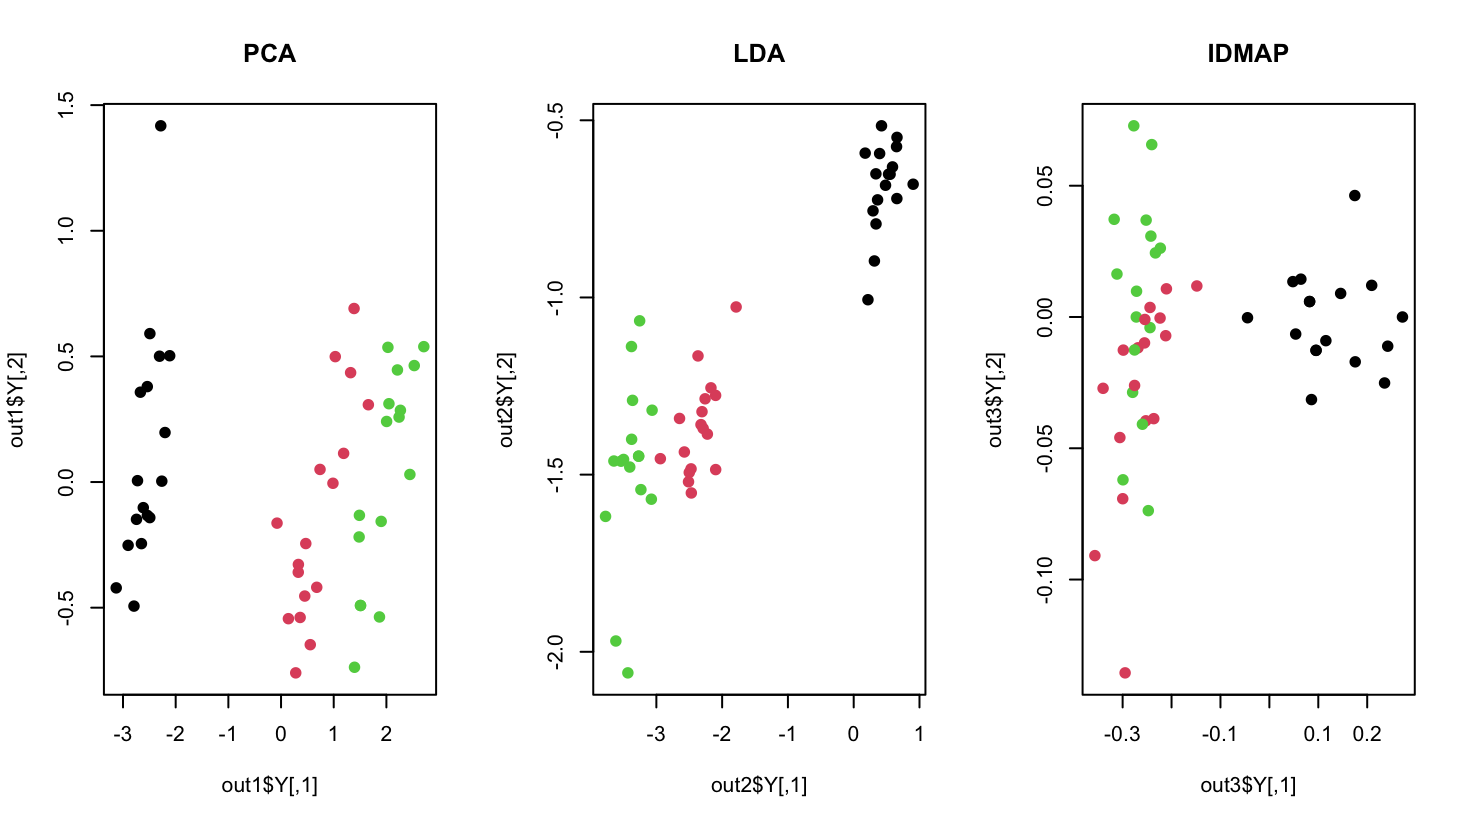
\includegraphics[width=0.8\textwidth]{figures/Rdimtools_test.png}
    \caption{Rdimtools test output.}
    \label{fig:rdimtools_test}
\end{figure}

\pagebreak
\section{Global versus local methods in nonlinear dimensionality reduction (\texorpdfstring{\cite{Silva2002}}{})}
\label{sec:deSilvaTenenbaum2002}

\subsection{Abstract}

\paragraph{Original:} Recently proposed algorithms for nonlinear dimensionality reduction fall broadly into two categories which have different advantages and disadvantages: global (Isomap), and local (Locally Linear Embedding, Laplacian Eigenmaps). We present two variants of Isomap which combine the advantages of the global approach with what have previously been exclusive advantages of local methods: computational sparsity and the ability to invert conformal maps.

\paragraph{Apple Intelligence summary:} Two new Isomap variants are presented, combining global advantages with local computational sparsity and conformal map inversion.

\subsection{Key Points}

\begin{itemize}
    \item \textbf{Introduction of LMDS} by applying it to Isomap (L-Isomap).
    \item \textbf{\textit{Landmark points}} $(n << N)$ reduce the complexity of computing:
    \begin{itemize}
        \item the distances matrix with Dijkstra's algorithm with Fibonacci heaps ($k$ = neighborhood size) from $\mathcal{O}(kN^2\log N)$ to $\mathcal{O}(knN\log N)$.
        \item MDS from $\mathcal{O}(n^3)$ to $\mathcal{O}(n^2N)$.
    \end{itemize}
    \item If $x$ is a landmark point, then the embedding given by LMDS is consistent with the original MDS embedding.
    \item If the distance matrix $D_{n,N}$ can be represented exactly by a Euclidean configuration in $\mathbb{R}^l$, and if the landmarks are chosen so that their affine span in that the configuration is $l$-dimensional (i.e. general position), then LMDS will recover the configuration exactly, up to rotation and translation.
\end{itemize}

\begin{figure}[ht]
    \centering
    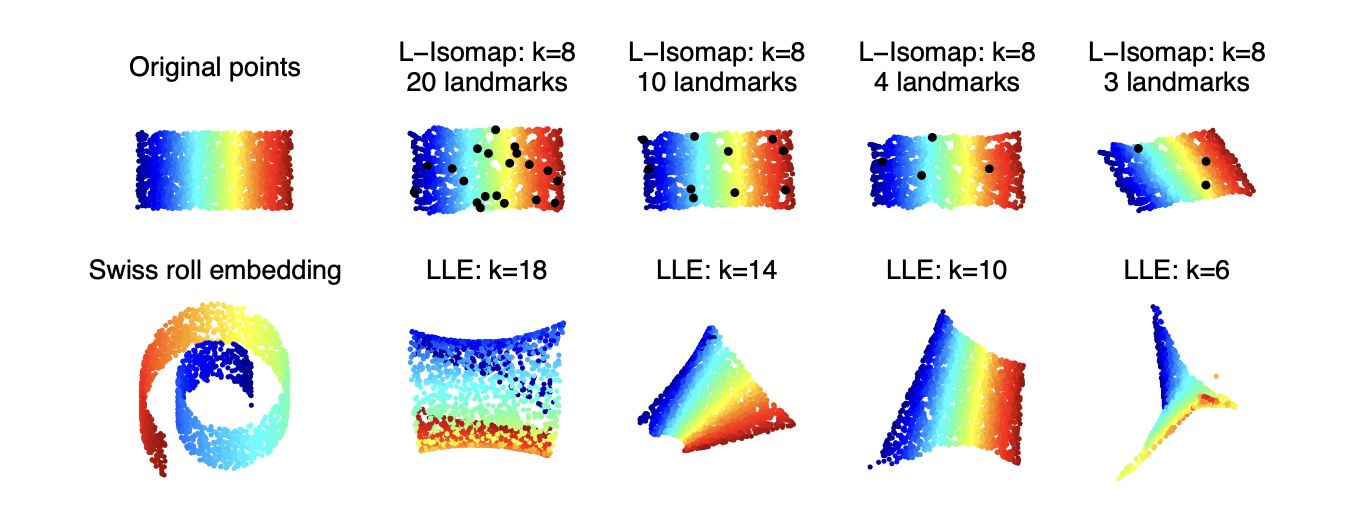
\includegraphics[width=0.8\textwidth]{figures/LMDS_3.png}
    \caption{L-Isomap is stable over a wide range of values for the sparseness parameter (the number of landmarks). Results from LLE are shown for comparision (\cite{Silva2002}).}
    \label{fig:LMDS}
\end{figure}


\pagebreak
\section{\texttt{dimRed} and \texttt{coRanking} - Unifying Dimensionality Reduction in R \texorpdfstring{\\ (\cite{Kraemer2018})}{}}
\label{sec:Kraemer2018dimRedAC}

\subsection{Abstract}

\paragraph{Original:} “Dimensionality reduction” (DR) is a widely used approach to find low dimensional and interpretable representations of data that are natively embedded in high-dimensional spaces. DR can be realized by a plethora of methods with different properties, objectives, and, hence, (dis)advantages. The resulting low-dimensional data embeddings are often difficult to compare with objective criteria. Here, we introduce the \texttt{dimRed} and \texttt{coRanking} packages for the R language. These open source software packages enable users to easily access multiple classical and advanced DR methods using a common interface. The packages also provide quality indicators for the embeddings and easy visualization of high dimensional data. The \texttt{coRanking} package provides the functionality for assessing DR methods in the co-ranking matrix framework. In tandem, these packages allow for uncovering complex structures high dimensional data. Currently 15 DR methods are available in the package, some of which were not previously available to R users. Here, we outline the \texttt{dimRed} and \texttt{coRanking} packages and make the implemented methods understandable to the interested reader.

\paragraph{Apple Intelligence summary:} Dimensionality reduction (DR) methods create low dimensional data representations, but comparison is challenging. The \texttt{dimRed} (figure \ref{fig:dimRed_methods}) and \texttt{coRanking} R packages are introduced to address this.

\subsection{Key Points}

\begin{itemize}
    \item The difficulty in applying DR is that each DR method is designed to maintain certain aspects of the original data and therefore may be appropriate for one task and inappropriate for another. Most methods also have parameters to tune and follow different assumptions.
    \item \textbf{Software packages for other languages}:
        \begin{itemize}
            \item Python: \texttt{scikit-learn}, which contains a module for DR.
            \item Julia: \texttt{ManifoldLearning.jl} for nonlinear and \texttt{MultivariateStats.jl} for linear DR.
            \item Matlab: several toolboxes.
            \item C++: \texttt{Shogun} toolbox, which offers bindings for many high level languages (including R).
        \end{itemize}
    \item At the time (2018), no comprehensive package for R.
    \item None of the former provides means to consistently compare the quality of different methods.
    \item MDS can be seen as kPCA with kernel $x^T y$, since a distance matrix can be transformed to a matrix of inner products.
    \item \texttt{dimRed} wraps \texttt{cmdscale}.
    \item In contrast to a supervised problem, there is no natural way to directly measure the quality of any output or to compare two methods. Every
    method optimizes a different error function.
    \item \textbf{Quality criteria implemented in \texttt{coRanking}}:
        \begin{itemize}
            \item \textbf{Co-ranking matrix based measures}: the co-ranking matrix $Q$ is the 2d-histogram of the distance ranks. $q_{ij}$ is an integer which counts how many points of distance rank $j$ became rank $i$. In a perfect DR, this matrix will only have non-zero entries in the
            diagonal. In R, the co-ranking matrix can be calculated using the the \texttt{coRanking::coranking} function. The \texttt{dimRed} package contains the functions \texttt{Q\_local, Q\_global, Q\_NX, LCMC}, and \texttt{R\_NX} to calculate the above quality measures in addition to \texttt{AUC\_lnK\_R\_NX}. If $R_{NX}$ is high for low values of $K$, then local neighborhoods are maintained well; if $R_{NX}$ is high for large values of $K$, then global gradients are maintained well (see figure \ref{fig:dimRed_R_NX}).
            \item Cophenetic correlation.
            \item \textbf{Reconstruction error}: the fairest one when the method provides an inverse mapping. $\mathrm{RMSE}=\sqrt{\frac{1}{n} \sum_{i=1}^n d\left(x_i^{\prime}, x_i\right)^2}$, with $x_i' = f^{-1}(y_i) = f^{-1}(f(x_i))$.
        \end{itemize}
    \item \textbf{Test datasets}: Common ones being the 3d S-curve and the Swiss roll. Real world examples usually have more dimensions and often are much noisier and we cannot be sure if we can observe all the relevant variables. Can be retrieved with \texttt{dimRed::loadDataSet}
    \item \textbf{Main functions:} \texttt{embed, quality, plot, plot\_R\_NX}.
\end{itemize}

\begin{figure}[ht]
    \centering
    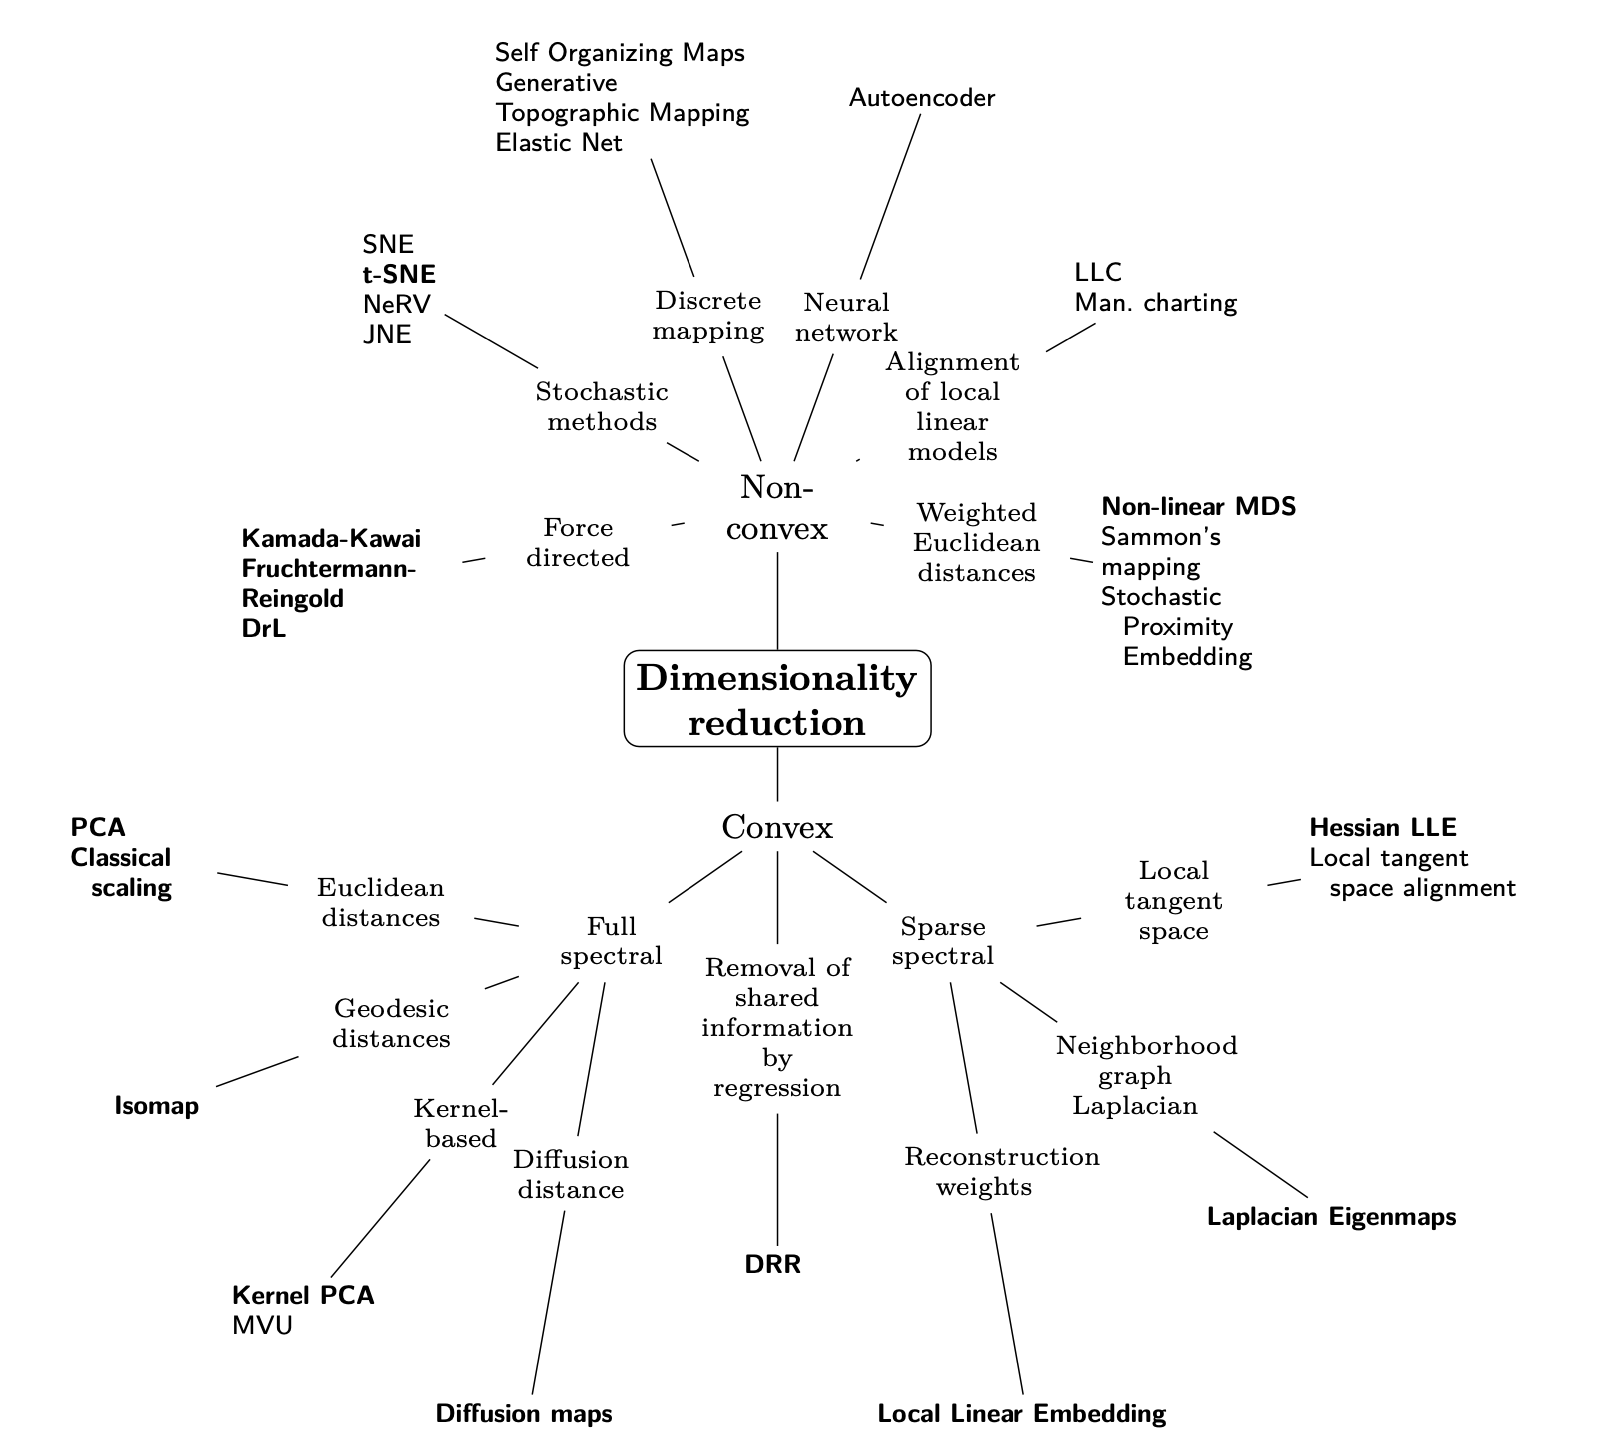
\includegraphics[width=0.8\textwidth]{figures/dimRed_methods.png}
    \caption{DR methods implemented in \texttt{dimRed} (\cite{Kraemer2018}).}
    \label{fig:dimRed_methods}
\end{figure}

\begin{figure}[ht]
    \centering
    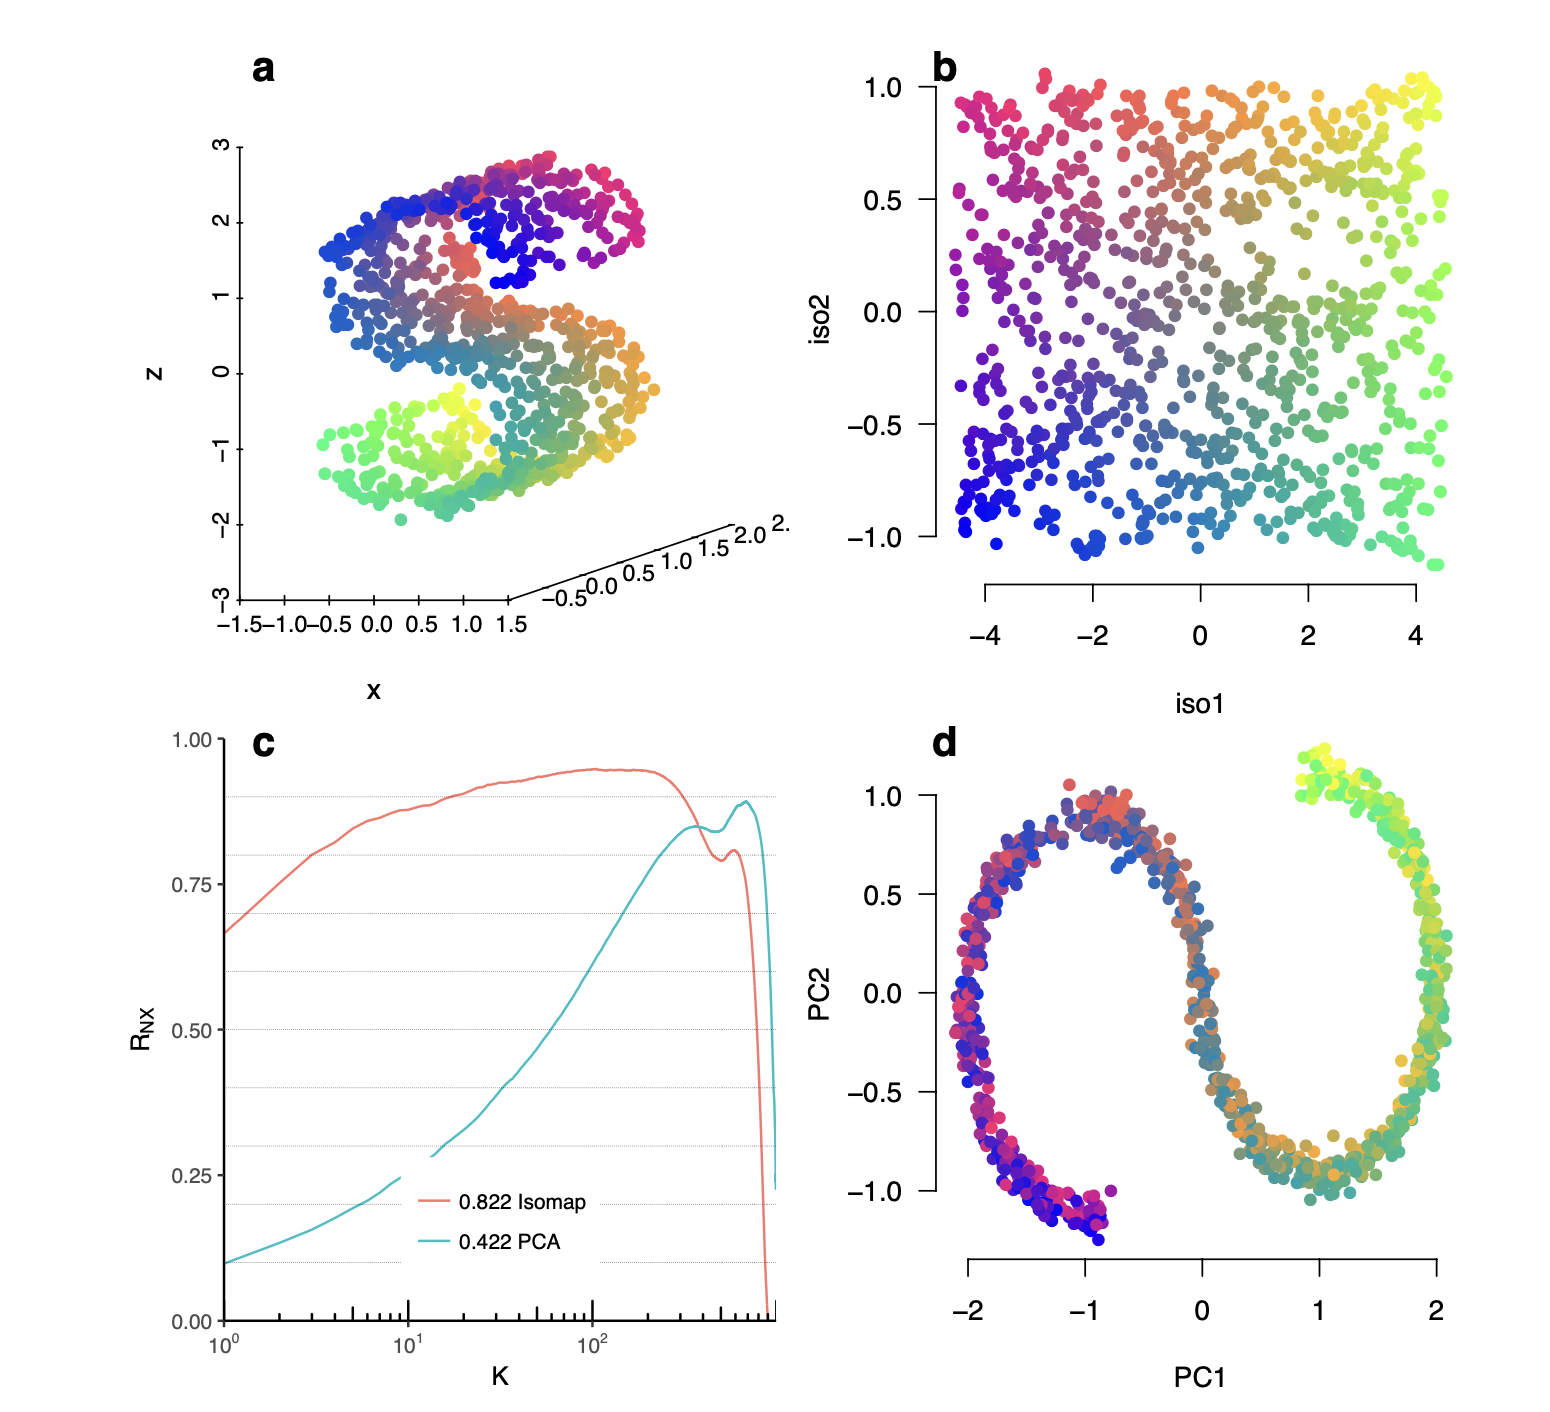
\includegraphics[width=0.8\textwidth]{figures/dimRed_R_NX.png}
    \caption{$R_{NX}$ measures the quality of the embedding. (\cite{Kraemer2018}).}
    \label{fig:dimRed_R_NX}
\end{figure}


\pagebreak
\section{Sparse multidimensional scaling
using landmark points (\texorpdfstring{\cite{DeSilva2004}}{})}
\label{sec:LMDS:2004}

\subsection{Abstract}

\paragraph{Original:} In this paper, we discuss a computationally efficient approximation to the classical multidimensional scaling (MDS) algorithm, called Landmark MDS (LMDS), for use when the number of data points is very large. The first step of the algorithm is to run classical MDS to embed a chosen subset of the data, referred to as the 'landmark points', in a low-dimensional space. Each remaining data point can be located within this space given knowledge of its distances to the landmark points. We give an elementary and explicit theoretical analysis of this procedure, and demonstrate with examples that LMDS is effective in practical use.

\paragraph{Apple Intelligence summary:} Landmark MDS approximates classical multidimensional scaling for large datasets. It embeds a subset of data points, called “landmark points”, in a low-dimensional space, then locates remaining points based on their distances to these landmarks.


\subsection{Key Points}

\begin{itemize}
    \item \textbf{LMDS}: Landmark MDS.
    \item \textbf{Method}:
        \begin{enumerate}
            \item Select $n$ landmark points from $N$ data points.
            \item Apply MDS to the $n \times n$ distance matrix to obrain $L$.
            \item Embed remaining points via distance-based triangulation.
        \end{enumerate}
    \item \textbf{Complexity}: Classical MDS: $\mathcal{O}(N^2)$ storage, $\mathcal{O}(N^3)$ time. LMDS: $\mathcal{O}(nN)$ storage, lower time complexity.
    \item It has links with Isomap (L-Isomap), the Nyström method (which finds approximate solutions to a positive semi-definite symmetric eigenvalue problem using just a few of the columns of the matrix) and FastMap.
\end{itemize}


\pagebreak
\section{Comparative study for dimensionality reduction techniques for big data (\texorpdfstring{\cite{Salah2020}}{})}
\label{sec:SalahHenouda2020}

\subsection{Abstract}

\paragraph{Original:} Nowadays, big data represents the solution for different type of users especially enterprises due to its huge amount of information augmented in real time. All these generated data could be described in one of big data characteristics named variety. One of the most challenging issues
for big data variety is high dimensionality because, it prevents the analysis process, demands heavy computations and adds noise to our data. The solution for this challenging issue is dimensionality reduction which minimize the dimensions and keeps only the essential information that give accurate results during analysis and decrease the computations complexity.

This paper aims to summarize and compare some of the recent methods that are used to solve the problem of high dimensionality in big data, Thereby, facilitating the process of research in this field.

\paragraph{Apple Intelligence summary:} High dimensionality in big data poses challenges, requiring dimensionality reduction to minimize dimensions and retain essential information. This paper compares recent methods for solving this problem, aiding research in the field.


\subsection{Key Points}

\begin{itemize}
    \item \textbf{Techniques Compared:}
        \begin{itemize}
            \item Classical/Modified PCA (modified to handle memory limits via row-scanning and MapReduce).
            \item Simplicial Nonnegative Matrix Tri-Factorization (SNMTF), an improved variant of NMF.
            \item Stacked Autoencoders, which yield lower reconstruction error than PCA.
            \item Linguistic Hedges Neuro-Fuzzy Classifiers with Feature Selection (LHNFCSF), a combination of neural networks and fuzzy inference systems (neuro-fuzzy) based on linguistic hedges with feature selection method.
            \item Deep Belief Networks (DBNs), which consist of multiple hidden layers where each layer is an RBM (Restricted Boltzmann Machine), which is also a class of neural networks. Each RBM is connected with two layers, a hidden layer and a visible layer, and so on.
        \end{itemize}
\end{itemize}


\pagebreak
\section{Out-of-Core Dimensionality Reduction for Large Data via Out-of-Sample Extensions (\texorpdfstring{\cite{Reichmann2024}}{})}
\label{sec:reichmann2024outofcoredimensionalityreductionlarge}

\subsection{Abstract}

\paragraph{Original:} Dimensionality reduction (DR) is a well-established approach for the visualization of high-dimensional data sets. While DR methods
are often applied to typical DR benchmark data sets in the literature, they might suffer from high runtime complexity and memory requirements, making them unsuitable for large data visualization especially in environments outside of high-performance computing. To perform DR on large data sets, we propose the use of out-of-sample extensions. Such extensions allow inserting new data into
existing projections, which we leverage to iteratively project data into a reference projection that consists only of a small manageable subset. This process makes it possible to perform DR out-of-core on large data, which would otherwise not be possible due to memory and runtime limitations. For metric multidimensional scaling (MDS), we contribute an implementation with out-of-sample projection capability since typical software libraries do not support it.

We provide an evaluation of the projection quality of five common DR algorithms (MDS, PCA, t-SNE, UMAP, and autoencoders) using quality metrics from the literature and analyze the trade-off between the size of the reference set and projection quality. The run-time behavior of the algorithms is also quantified with respect to reference set size, out-of-sample batch size, and dimensionality of the data sets. Furthermore, we compare the out-of-sample approach to other recently introduced DR methods, such as PaCMAP and
TriMAP, which claim to handle larger data sets than traditional approaches. To showcase the usefulness of DR on this large scale, we contribute a use case where we analyze ensembles of streamlines amounting to one billion projected instances.

\paragraph{Apple Intelligence summary:} The study compares out-of-sample DR methods with PaCMAP and TriMAP on large datasets.  A use case demonstrates the usefulness of DR on a dataset of one billion projected streamline instances.

\subsection{Key Points}

\begin{itemize}
    \item A framework for OOS extensions of DR methods similar to Interpolation MDS.
    \item Applied to PCA, MDS, t-SNE, UMAP and autoencoders.
    \item Compared to TriMap and PaCMAC, which are efficient DR methods suitable for big data.
    \item \textbf{Related work}:
    \begin{itemize}
        \item \textbf{Efficient DR algorithms}: PaCMAP (up to 4 million data points), TriMAP (up to 11 million data points), LargeVis (also millions of data points, aimed to reduce computational cost of t-SNE). Note that t-SNE and UMAP fail at 1 million data points.
        \item \textbf{Parametric DR methods}: learn explicit maps between the high- and low-dimensional space.  Hinterreiter et al. (\cite{Hinterreiter2023}) introduced a framework making parametric extensions generally available for DR techniques.
        \item \textbf{GPU porting}: of t-SNE, UMAP and metrics computations such as trustworthiness. Reichmann et al. also parallelize metric MDS.
        \item \textbf{OOS extensions}: Bengio et. al. (\cite{Bengio2003})introduced an OOS framework by learning the corresponding eigenfunctions. Gisbrecht et. al. (\cite{Gisbrecht2012}) proposed three kernel-based methods and (\cite{Zhang2021}) improved them.
    \end{itemize}
    \item \textbf{Computational framework}: see figure \ref{fig:OOS_algorithm}. Details and sematics of the $\beta$ parameters depends on the DR method. As an example, see figure \ref{fig:OOS_methods}.
    
    \begin{figure}[ht]
        \centering
        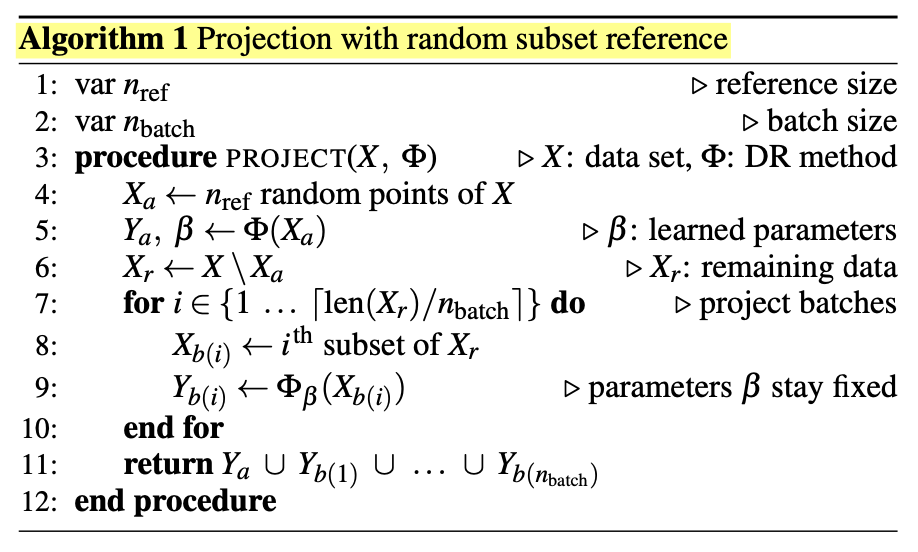
\includegraphics[width=0.8\textwidth]{figures/OOS_algorithm.png}
        \caption{OOS projection framework proposed in (\cite{Reichmann2024}).}
        \label{fig:OOS_algorithm}
    \end{figure}

    \begin{figure}[ht]
        \centering
        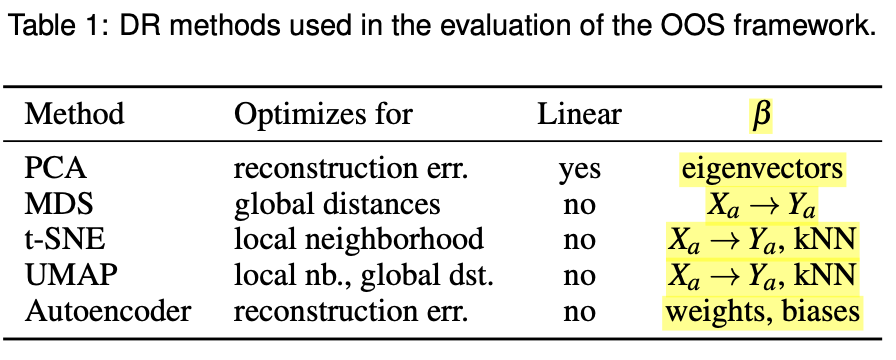
\includegraphics[width=0.8\textwidth]{figures/OOS_methods.png}
        \caption{DR methods used in the evaluation of the OOS framework proposed in (\cite{Reichmann2024}).}
        \label{fig:OOS_methods}
    \end{figure}

    \item \textbf{OOS extensions} used:
    \begin{itemize}
        \item \textbf{PCA} and the \textbf{autoencoder} learn a parametric mapping and give an explicit function to map the data.
        \item For \textbf{metric MDS}, they minimize stress for a single point while keeping all others fixed (\textit{single scaling}) to perform the OOS projection of a single point. The gradient for an OOS point $x^{\prime}$ with respect to the points $x_i$ of the reference set $X_a$ and corresponding low-dimensional points $y_i$ is given as $\delta=\sum_i\left(1-d\left(x^{\prime}, x_i\right) /\left\|y^{\prime}-y_i\right\|\right) \cdot\left(y^{\prime}-y_i\right)$, with dissimilarity function $d(\cdot, \cdot)$. We have run the code provided in the article with a Windows system that has an NVIDIA graphics card and obtained the results shown in figure \ref{fig:CUDA_MDS}. Details can be found on \verb$code/ReichmanHagele2024_MDS/mds_demo.py$.

        \begin{figure}[ht]
            \centering
            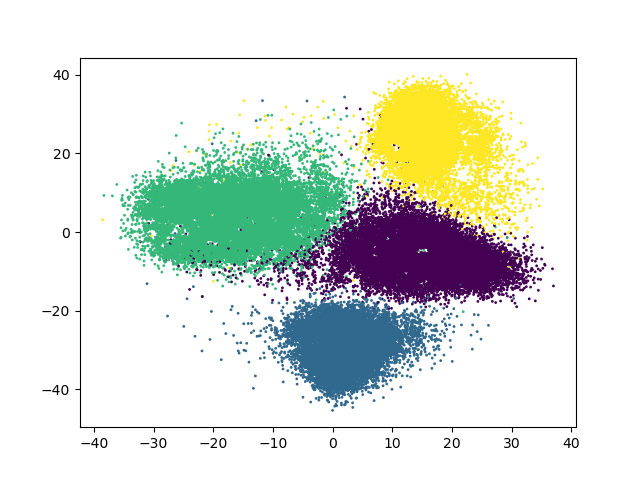
\includegraphics[width=0.8\textwidth]{figures/CUDA_MDS.png}
            \caption{Output of the CUDA imeplementation in (\cite{Reichmann2024}) of metric MDS for a test dataset.}
            \label{fig:CUDA_MDS}
        \end{figure}
        
        \item A similar mechanism can be used in \textbf{t-SNE} and \textbf{UMAP}.
    \end{itemize}
    \item \textbf{Datasets} of up to 50,000,000 data points were used to evaluate the OOS framework, as can be seen in figure \ref{fig:OOS_datasets}. That being said, a non-consumer very powerful system was used; it consisted of an AMD Ryzen Threadripper PRO 3995WX with 64 CPU cores, an NVIDIA RTX A6000 GPU with 48 GiB of VRAM, and 251 GiB of RAM.
    
    \begin{figure}[ht]
        \centering
        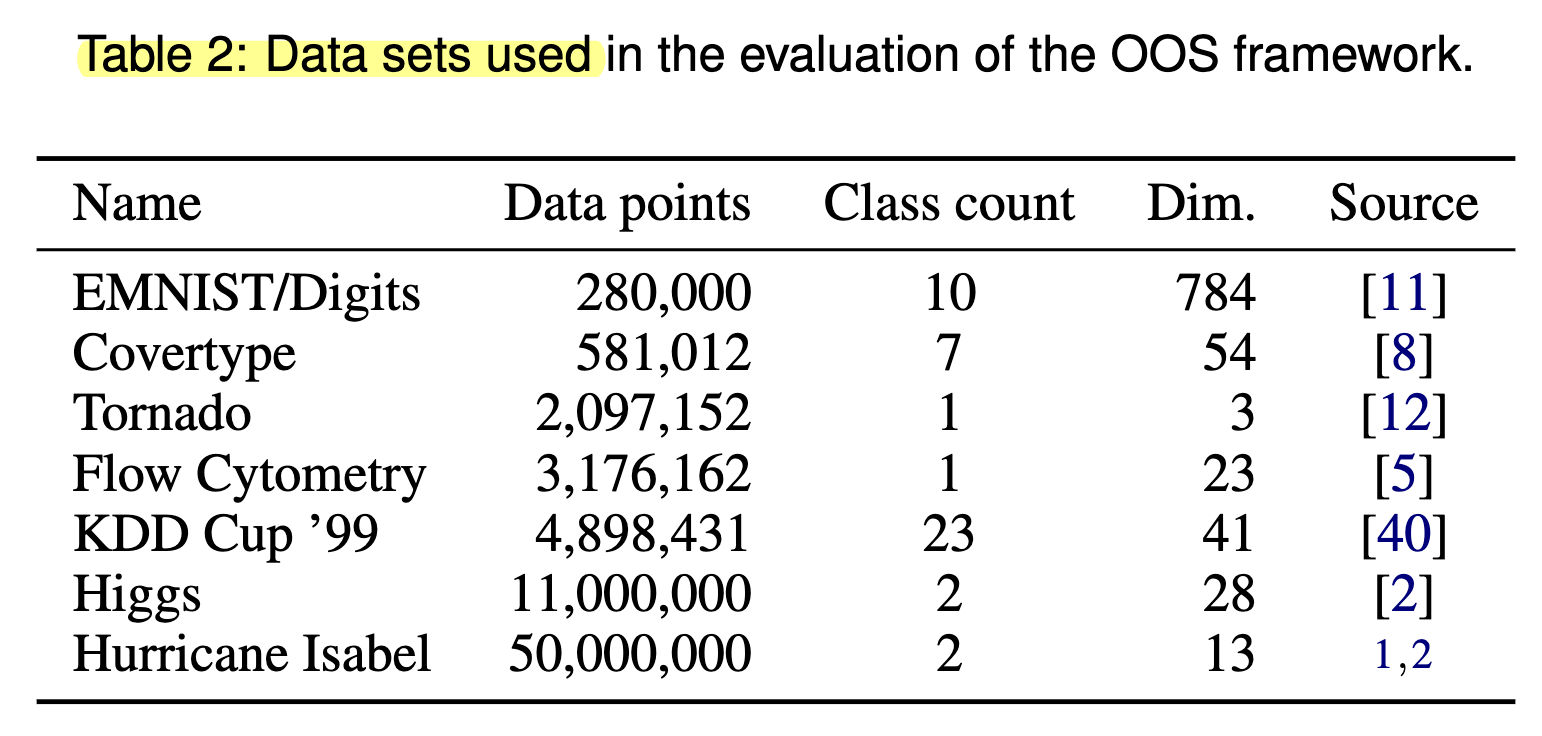
\includegraphics[width=0.8\textwidth]{figures/OOS_datasets.png}
        \caption{Datasets used in the evaluation of the OOS framework proposed in (\cite{Reichmann2024}).}
        \label{fig:OOS_datasets}
    \end{figure}
    
    \item \textbf{Metrics} used:
    \begin{itemize}
        \item \textbf{Global}: \textit{stress} (calculation in batches in the GPU), \textit{Pearson correlation coefficient} between the flattened low- and high-dimensional distance vectors.
        \item \textbf{Local}: \textit{KNN precision}, \textit{trustworthiness} (calculation in batches in the GPU).
    \end{itemize}
    
    \item \textbf{Computational complexities}:
    \begin{itemize}
        \item Runtime (RT) complexity:
        $\mathcal{O}\Bigl(\Phi^{\mathrm{RT}}\bigl(n_{\mathrm{ref}}\bigr)\Bigr)
        +\mathcal{O}\Bigl(\Phi_\beta^{\mathrm{RT}}\bigl(n_{\mathrm{batch}}\bigr)
        \cdot \text{batch\_count}\Bigr)$
        \item Memory (M) complexity of a batch projection:
        $\mathcal{O}\Bigl(\Phi^{\mathrm{M}}\bigl(n_{\mathrm{ref}}\bigr)\Bigr)
        +\mathcal{O}\Bigl(\Phi_\beta^{\mathrm{M}}\bigl(n_{\mathrm{batch}}\bigr)\Bigr)$
        \item Metric MDS: $\Phi\bigl(n_{\mathrm{ref}}\bigr)$ is $\mathcal{O}(n_{\mathrm{ref}}^2)$ in RT and M. $\Phi_{\beta}\bigl(n_{\mathrm{batch}}\bigr)$ has $\mathcal{O}(n_{\mathrm{ref}} \cdot n_{\mathrm{batch}})$ time complexity (and I'd argue it is $\mathcal{O}(n_{\mathrm{batch}}^2)$ in memory).
        \item t-SNE: same as metric MDS, except for M of $\Phi_{\beta}$.
        \item UMAP: $\Phi\bigl(n_{\mathrm{ref}}\bigr)$ is $\mathcal{O}(n_{\mathrm{ref}}^{1.14})$ in T and $\Phi_{\beta}\bigl(n_{\mathrm{batch}}\bigr)$ is like in MDS.
        \item Autoencoders: $\Phi$ has linear TR and its M depends on the architecture. $\Phi_{\beta}$ is approximately linear.
        \item PCA: $\Phi$ is linear with respect to $n_{\mathrm{ref}}$ and dimensionality. $\Phi_{\beta}$ is approximately linear.
    \end{itemize}

    \item \textbf{Implementation}: in Python with \texttt{Numba}(see section \ref{sec:Numba}) compiled functions for performance-critical sections. They used the UMAP implementation of the umap-learn library, the openTSNE library for t-SNE, scikit-learn for PCA, and keras for the autoencoder. For MDS, they provided their own implementation (see \verb$code/ReichmanHagele2024_MDS/mds_demo.py$).
    \item \textbf{Experiments results}:
    \begin{itemize}
        \item \textbf{Quality}: PCA and MDS are consistent very early on (starting with a ref. set size of 128). t-SNE and UMAP overfit and generate clusters on small ref. sets, although they perform well on local metrics. Autoencoders is the most inconsistent method, but in general when the ref. set size increases, global metrics worsen and local ones improve.
        \item \textbf{Runtime}: PCA and MDS are consistent with theory. t-SNE shows a below quadratic time complexity of $\Phi$, why? Moreover, time complexity of $\Phi_{\beta}$ seems constant with respect to $n_{\mathrm{ref}}$, why? UMAP is significantly slower in high-dimensional datasets. The dependance on batch size is inconsistent in most methods, even though the general trend is to be sub-linear.
    \end{itemize}
    \item \textbf{Comparison to large-scale DR methods}: when comparing UMAP with the proposed OOS framework against classical UMAP, PaCMAP and TriMap, PaCMAP is consistently better in terms of quality metrics, although the OOS framework is capable of reducing runtime significantly at the expense of quality. In previous work, UMAP failed to transform datasets of 1 million rows; how did the authors manage to run it on datasets of 2, 5 and 11 million data points (Tornado, KDD Cup '99 and Higgs, respectively)?

    \item They finally show a use case with 1 billion streamlines generated on the \textit{fluid simulation ensemble for machine learning}.
    
    \item \textbf{Final discussion}:
    \begin{itemize}
        \item Even though results depend on the DR technique, runtime can always be substantially reduced by using smaller reference set sizes.
        \item The authors recommend testing the reference projection before applying the OOS projection to the whole data set.
        \item Tuning the hyperparameters of the DR methods should improve results.
        \item An informed selection of the reference set instead of a random one could improve results as well.
        \item Another limitation of the proposed framework is that relationships between OOS points are ignored and that $\Phi_{\beta}$ is not updated with OOS points.
    \end{itemize}
\end{itemize}


\pagebreak
\section{Local Multidimensional Scaling for Nonlinear Dimension Reduction, Graph Drawing, and Proximity Analysis (\texorpdfstring{\cite{Chen2009}}{})}
\label{sec:LocalMDS}

\subsection{Abstract}

\paragraph{Original:} In the past decade there has been a resurgence of interest in nonlinear dimension reduction. Among new proposals are "Local Linear Embedding", "Isomap", and Kernel Principal Components Analysis which all construct global low-dimensional embeddings from local affine or metric information. We introduce a competing method called "Local Multidimensional Scaling" (LMDS). Like LLE, Isomap, and KPCA, LMDS constructs its global embedding from local information, but it uses instead a combination of MDS and "force-directed" graph drawing. We apply the force paradigm to create localized versions of MDS stress functions with a tuning parameter to adjust the strength of nonlocal repulsive forces. We solve the problem of tuning parameter selection with a meta-criterion that measures how well the sets of K-nearest neighbors agree between the data and the embedding. Tuned LMDS seems to be able to outperform MDS, PCA, LLE, Isomap, and KPCA, as illustrated with two well-known image datasets. The meta-criterion can also be used in a pointwise version as a diagnostic tool for measuring the local adequacy of embeddings and thereby detect local problems in dimension reductions.

\paragraph{Apple Intelligence summary:} Tuned LMDS outperforms other dimension reduction methods on image datasets.  LC meta-criteria measure agreement between data and embedding, aiding tuning and detecting local problems.

\subsection{Key Points}

\begin{itemize}
    \item The stability of optimal MDS configurations stems from the large dissimilarities, and localized MDS did not appear to be a viable approach. \item In view of MDS' reliance on large distances, Isomap may be driven mostly by the large but noisy shortest-path imputations, whereas the local distances play only a minor role.
    \item Isomap suffers from more variance, LLE and LMDS from more bias.
    \item LC meta-criteria are proposed and used to tune parameters and to produce diagnostic plots. However, they are not smooth and statistically unstable.
    \item \textbf{LMDS}: given a distance matrix $D_{i,j}$, let $\mathcal{N}$ be a symmetrized k-NN graph: $(i,j)\in\mathcal{N}$ if $j$ is among the $K$ nearest neighbors of $i$ or viceversa. LMDS looks for a low-dimensional configuration $\mathbf{x}_1, \dots, \mathbf{x}_N \in \mathbb{R}^d$ that minimizes
    $$
    \operatorname{LMDS}_{\mathcal{N}}^D\left(\mathbf{x}_1, \ldots, \mathbf{x}_N\right)= \sum_{(i, j) \in N}\left(D_{i, j}-\left\|\mathbf{x}_i-\mathbf{x}_j\right\|\right)^2 - t \sum_{(i, j) \notin N}\left\|\mathbf{x}_i-\mathbf{x}_j\right\|,
    $$
    with $t=\frac{|\mathcal{N}|}{\left|\mathcal{N}^C\right|} \cdot \operatorname{median}_{\mathcal{N}}\left(D_{i, j}\right) \cdot \tau$.

    The first term is the "local stress" and the segond one is the "repulsion".

    A good strategy for optimization is to start with a large value such as $\tau = 1$ to obtain a stable configuration, and lower $\tau$ successively as low as 0.01, using previous configurations as initializations for smaller values of $\tau$.

    \item \textbf{LCMC (Local Continuity Meta-Criteria)}: For case $i$ we form the index set $\mathcal{N}_{K^{\prime}}^D(i)=\left\{j_1, \ldots, j_{K^{\prime}}\right\}$ of $K^{\prime}$-NNs with regard to $D_{i, j}$, and $\mathcal{N}_{K^{\prime}}^X(i)=\left\{k_1, \ldots, k_{K^{\prime}}\right\}$ of $K^{\prime}-$ NNs with regard to $\left\|\mathbf{x}_i-\mathbf{x}_k\right\|$ (excluding $i$ ). The overlap is measured pointwise and globally by
    $$
    N_{K^{\prime}}(i)=\left|\mathcal{N}_{K^{\prime}}^D(i) \cap \mathcal{N}_{K^{\prime}}^X(i)\right|, \quad N_{K^{\prime}}=\frac{1}{N} \sum_{i=1}^N N_{K^{\prime}}(i).
    $$

    Maximum faithfulness is achieved when $N_{K'} = K'$, so we normalize:
    $$
    M_{K'} = \frac{N_{K'}}{K'}.
    $$

    If there is complete absence of association between the data and the configuration, the local overlap $N_{K'}(i)$ is random and can be modeled by a hypergeometric with $\mathbb{E}[N_{K'}] = \frac{K'^2}{N-1}$. Hence, we define the \textit{adjusted LC meta-criteria} as:
    $$
    M_{K^{\prime}}^{\mathrm{adj}}=M_{K^{\prime}}-\frac{K^{\prime}}{N-1} .
    $$

    \item Selection of tuning parameters:
    \begin{itemize}
        \item $\mathbf{\tau}$: Given $K$ for LMDS$_{K,\tau}$ and $K'$ for $M_{K'}$, we can optimize the repulsion weight $\tau$ with a grid search. That is, for a set of $\tau$ values, we perform LMDS$_{K,\tau}$ and compute $M_{K'}$ on the obtained embeddings. Then, we choose the value for $\tau$ that maximizes $M_{K'}$.
        \item $K$: there are two strategies:
        \begin{itemize}
            \item $K'=K$: For fixed $K$ minimize $\operatorname{LMDS}_{K, \tau}$ for various values of $\tau$; pick the $\tau$ whose configuration maximizes $M_{K^{\prime}}^{\text {adj }}$; repeat for various values of $K=K^{\prime}$ and pick that $K=K^{\prime}$ which maximizes the trace.
            \item $K^{\prime}, K$ decoupled: It is desirable that $K$ is not just $M_{K^{\prime}}^{\text {adj }}$-optimal for $K^{\prime}=K$, but for a range of values $K^{\prime}$. To find out, one may plot traces $K^{\prime} \mapsto M_{K^{\prime}}^{\text {adj }}$ one for each value of $K$.
        \end{itemize}
    \end{itemize}

    \item The LC meta-criteria are doubly "non-metric" in the sense that they only use rank information of both $\{D_{i,j}\}$ and $\{\lVert x_i-x_j \rVert\}$.
    \item The Achilles heel of methods considered here is the complete reliance on distance data or dissimilarities, which holds both for the LMDS fitting criterion and the LC meta-criteria. This means that users might have to choose specific distances/dissimilarities for their problems.
    
\end{itemize}


\pagebreak
\section{Classical MDS benchmarked in R}

In this section we aim to test the limits of \texttt{Rdimtools::do.mds}. Specifically, we will run Rdimtools's implementation of Classical MDS on datasets of increasing number of observations and dimensionality in order to test its limitations as well as its complexity. We will also compare it with \texttt{dimRed::embed(.method="MDS", ...)}.

Code, data and figures of the experiment can be found in \verb$code/MDS_benchmark_R_lib$. As for the system used, tests were performed on a Macbook Pro (14-inc, Nov 2023) with 16 GB of RAM and the Apple M3 chip.

In our first experiment (see figure \ref{fig:MDS_Rdimtools}), we run \texttt{Rdimtools::do.mds} on datasets consisiting of four isotropic gaussian blobs with random covariance matrices randomly centered in a $d$-dimensional space with sizes ranging from 100 to 100000. We let $d$ be 8, 32 and 64. However, for all dimensionalities tested, R crashed when the dataset had at least 56234 rows. This result shows the memory limitation of classical MDS, which is reached in datasets with sizes of the order of $10^5$ for modern consumer-grade systems.

Regarding time complexity, classical MDS shows quadratic growth with respect to number of individuals and linear growth in dimensionality, although we cannot be absolutely sure of the latter because only three dimensionalities were tested.

\begin{figure}[ht]
    \centering
    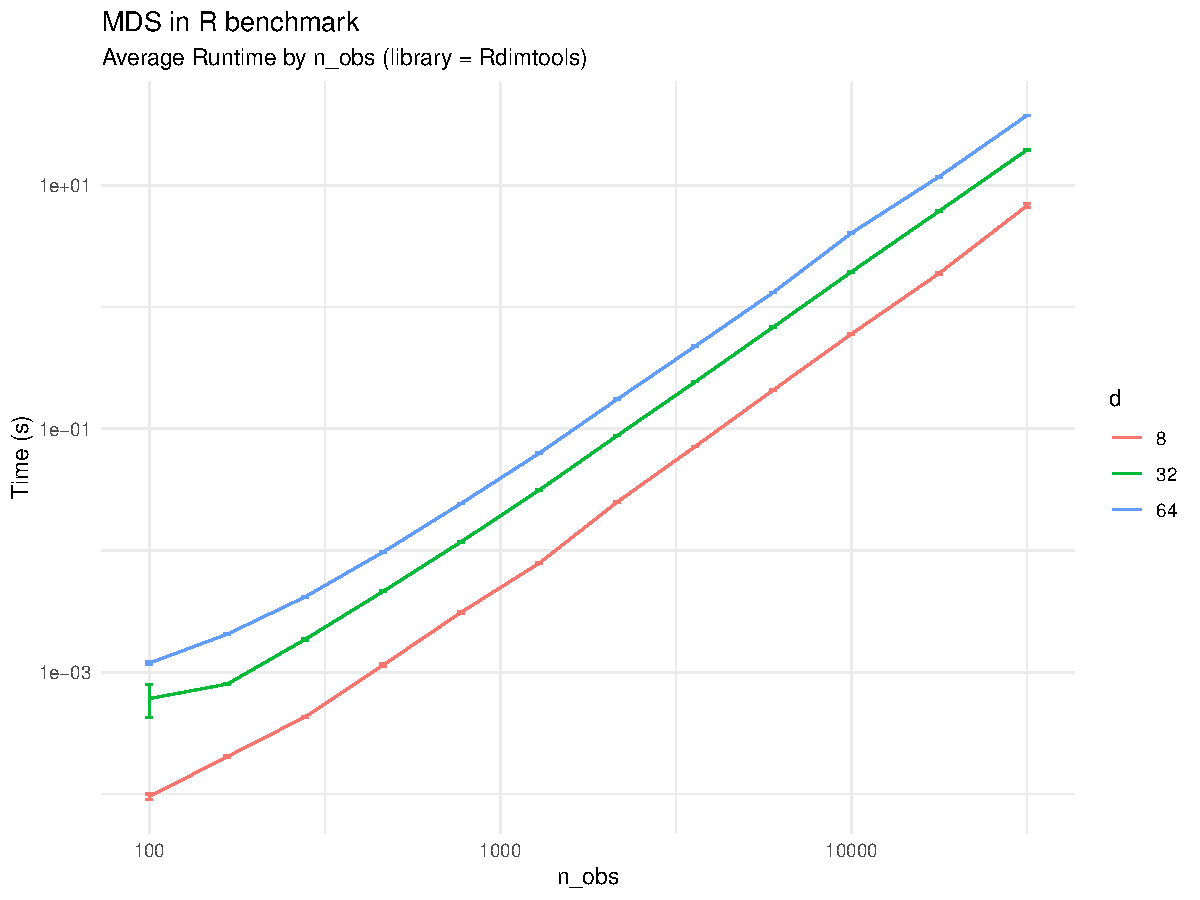
\includegraphics[width=0.8\textwidth]{figures/MDS_Rdimtools.pdf}
    \caption{Runtime (s) of \texttt{Rdimtools::do.mds} averaged over 20 experiments. The tests were performed on datasets consisiting of four isotropic gaussian blobs with random covariance matrix and randomly centered in a $d$-dimensional space with sizes ranging from 100 to 31623. We let $d$ be 8, 32 and 64.}
    \label{fig:MDS_Rdimtools}
\end{figure}

Next, we compared the implementations of classical MDS in libraries \texttt{Rdimtools} and \texttt{dimRed}, since \texttt{Rdimtools} is said to be very efficient while \texttt{dimRed} just wraps the \texttt{cmdscale} method (\cite{Kraemer2018}). As can be seen in figure \ref{fig:MDS_dimRed_vs_Rdimtools}, our tests corroborate the results shown in (\cite{You2022}), since \texttt{Rdimtools::do.mds} has a lower time complexity than \texttt{dimRed::embed(.method="MDS", ...)}, resulting in runtime improvements of 10x for datasets with 100 rows and up to 1000x for samples with 10000 observations. Indeed, we did not test \texttt{dimRed::embed(.method="MDS", ...)} on larger datasets because, when size equaled 1000 rows, each experiment took around 15 minutes to run on our system.

\begin{figure}[ht]
    \centering
    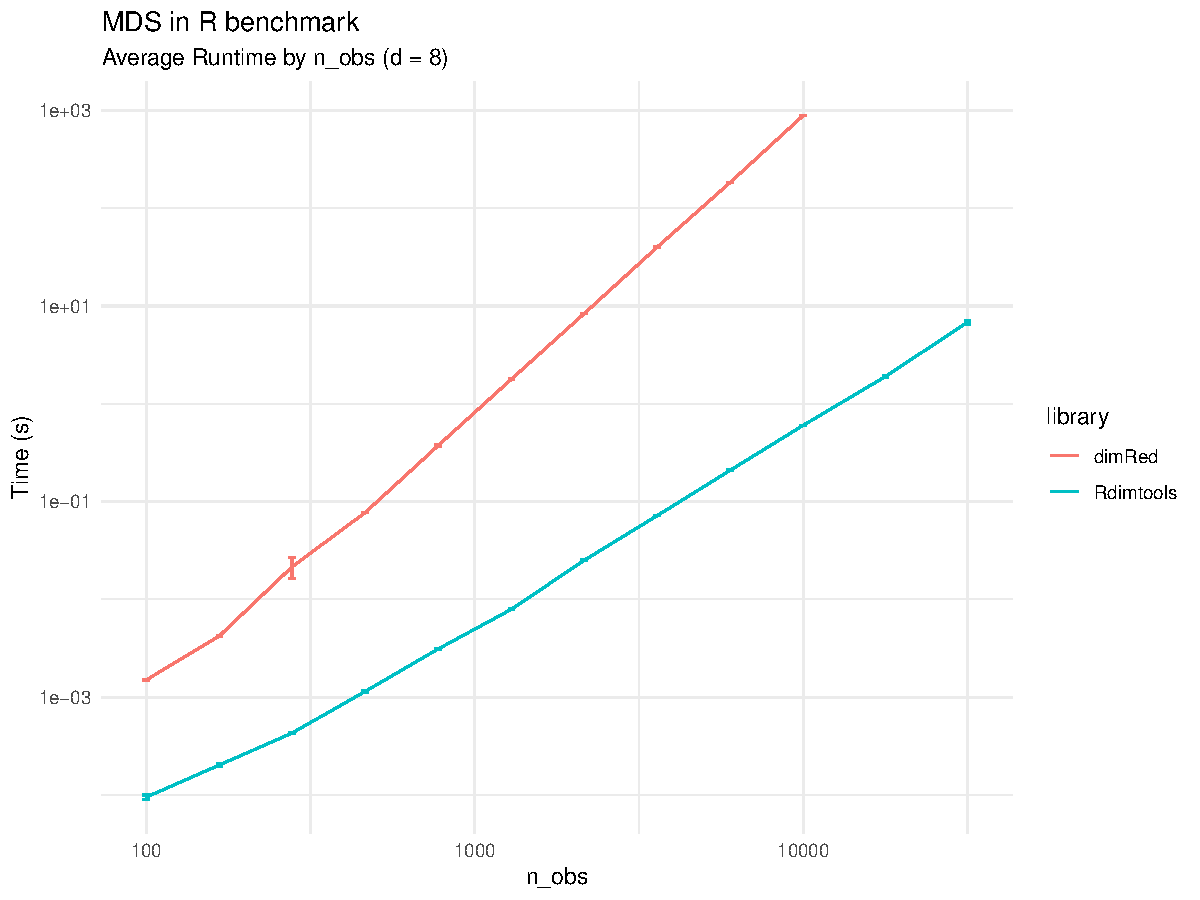
\includegraphics[width=0.8\textwidth]{figures/MDS_dimRed_vs_Rdimtools.pdf}
    \caption{Runtime (s) of \texttt{Rdimtools::do.mds} and \texttt{dimRed::embed(.method="MDS", ...)} averaged over 20 experiments. Both methods were tested on the same datasets, consisiting of four isotropic gaussian blobs with random covariance matrix and randomly centered in an 8-dimensional space with sizes ranging from 100 to 10000 for \texttt{dimRed::embed(.method="MDS", ...)} and from 100 to 31623 for \texttt{Rdimtools::do.mds}.}
    \label{fig:MDS_dimRed_vs_Rdimtools}
\end{figure}

\pagebreak
\section{DR Python packages}

\subsection{Key Points}

\begin{itemize}
    \item To our knowledge, there is no comprehensive Python package that implements many DR techniques akin the R library \texttt{Rdimtools} (see section \ref{sec:rdimtools}).
    \item To show the consequences of this in an example, classical MDS is only implemented in \texttt{pyseer} (through \texttt{pyseer.cmdscale}), a package for microbial pangenome-wide association studies (\cite{Lees2018}).
    \item The package that contains the most DR methods is \texttt{scikit-learn}, specifically in its \texttt{manifold} module (\cite{Pedregosa2011}). It implements: Isomap, LLE, Laplacian Eigenmaps, t-SNE and non-classical MDS (both \texttt{sklearn.manifold.MDS} and \texttt{sklearn.manifold.smacof} can perform metric and non-metric MDS). Moreover, \texttt{sklearn.manifold.trustworthiness} measures to what extent the local structure is retained when dimensionality is reduced. Hence, the total amount of methods present in \texttt{sklearn.manifold} cannot be compared to the 143 of \texttt{Rdimtools}.
    \item Another remarkable, although differently oriented, library is \texttt{direpack}, which implements a set of modern statistical dimension reduction techniques including projection pursuit, sufficient dimension reduction, and robust M estimators. It also includes regularized regression estimators, pre-processing utilities, plotting functionality, and cross-validation utilities, all consistent with the scikit-learn API (\cite{Menvouta2023}). Nonetheless, these methods are outside the scope of our thesis.
    \item Other, more specific, libraries that implement DR methods in Python are:
    \begin{itemize}
        \item \texttt{umap-learn}: the library that introduced UMAP (\cite{McInnes2018}).
        \item \texttt{MulticoreTSNE}: a multicore modification of Barnes-Hut t-SNE with Python CFFI-based wrappers (\cite{Ulyanov2016}). Barnes-Hut is a tree-based algorithm that can be used to accelerate t-SNE up to $\mathcal{O}(N\log N)$ (\cite{Vandermaaten2014}).
        \item \texttt{fitsne}: Fast Fourier Transform-accelerated Interpolation-based t-SNE (\cite{Linderman2019}).
        \item \texttt{OpenTSNE}: incorporates the latest improvements to the t-SNE algorithm, including the ability to add new data points to existing embeddings, massive speed improvements, enabling t-SNE to scale to millions of data points and various tricks to improve global alignment of the resulting visualizations \cite{Policar2024}. The team behind \texttt{OpenTSNE} benchmarked the here described t-SNE Python implementations and showed that the fastest one in general is \texttt{fitsne}, although \texttt{OpenTSNE} is equally efficient on multicore systems (see figure \ref{fig:python_tsne_benchmarks}) \cite{Policar2024}.
    \end{itemize}
    \item Moreover, other libraries focused on certain fields like genomics (\texttt{phate}) or NLP (\texttt{gensim}) implement DR methods for specific tasks and scenarios in their topics.
\end{itemize}

\begin{figure}[ht]
    \centering
    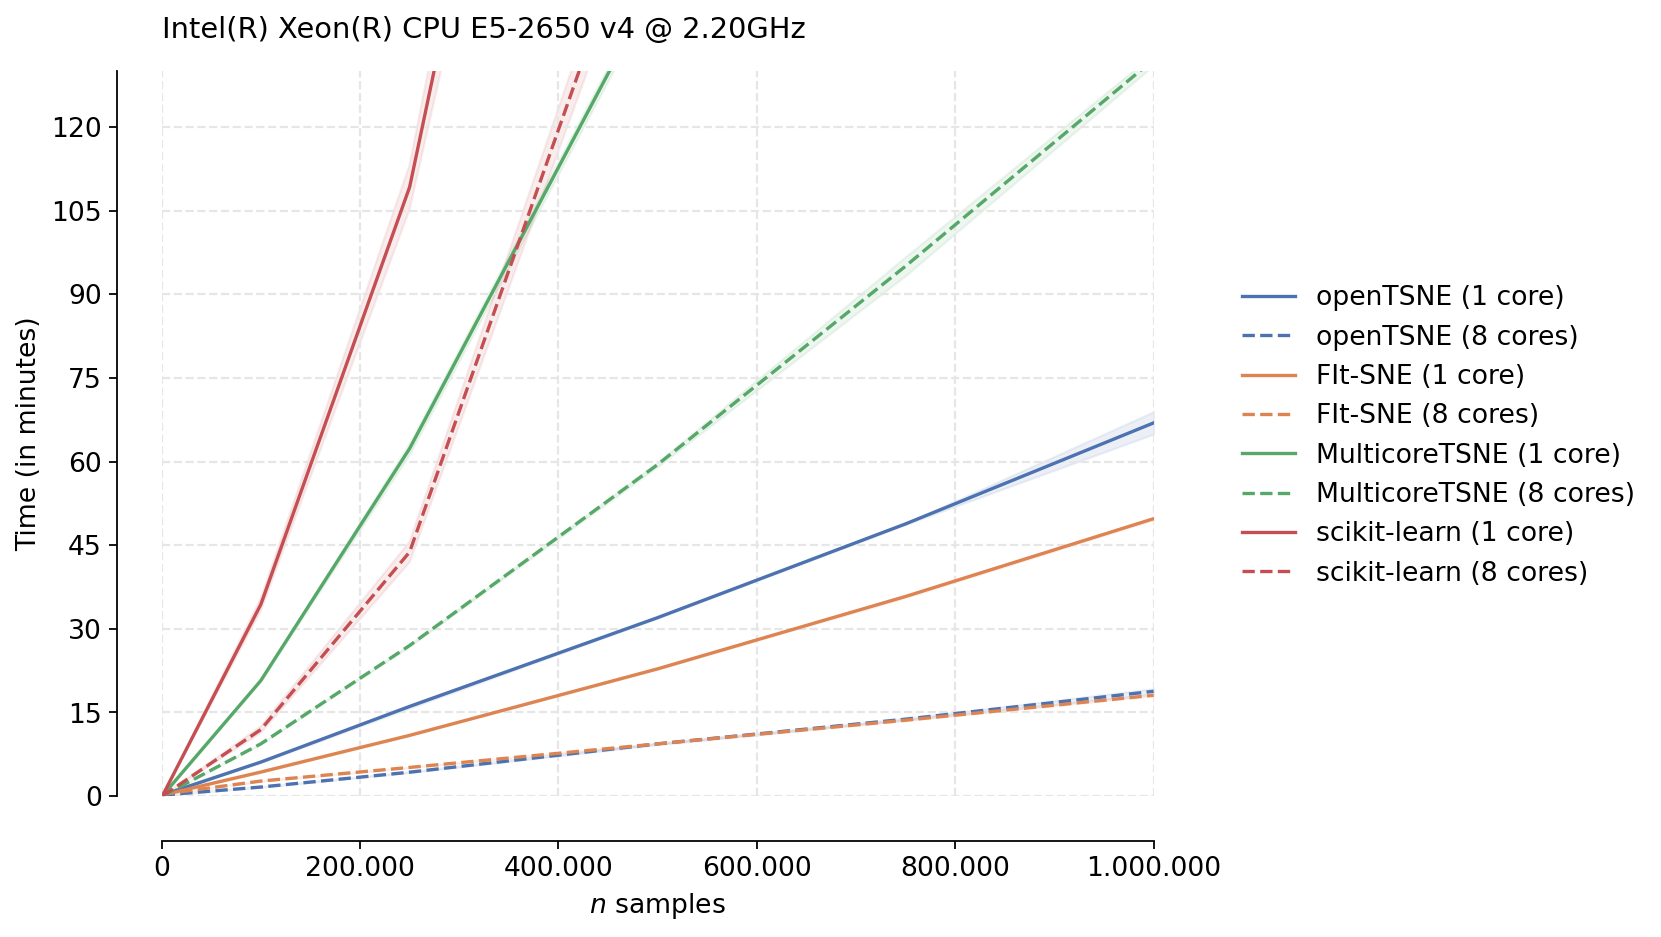
\includegraphics[width=0.8\textwidth]{figures/python_tsne_benchmarks.png}
    \caption{Benchmark of t-SNE Python implementations \cite{Policar2024}.}
    \label{fig:python_tsne_benchmarks}
\end{figure}

\pagebreak
\section{The \texttt{Numba} Python package}
\label{sec:Numba}

\texttt{Numba} (\cite{Lam2015}) is an open‐source just-in-time (JIT) compiler that translates a subset of Python and \texttt{Numpy} code into optimized machine code using LLVM.

It accelerates numerical computations on CPUs and GPUs by enabling parallelization and vectorization with minimal code modifications. To gain the most out of it, computations should use loops, \texttt{Numpy} functions and \texttt{Numpy} broadcasting.

\subsection{How does \texttt{Numba} work?}

As described in its documentation (\cite{Lam2015}), \texttt{Numba} reads the Python bytecode for a decorated function and combines this with information about the types of the input arguments to the function. It analyzes and optimizes your code, and finally uses the LLVM compiler library to generate a machine code version of your function, tailored to your CPU capabilities. This compiled version is then used every time your function is called.

\pagebreak
\section{Isomap in Python}

In this section we will explore the current Isomap Python implementations to use them later in our divide-and-conquer and recursive big data algorithms.

\subsection{Package implementations}

\begin{itemize}
    \item \texttt{sklearn.manifold.Isomap} (see \cite{Pedregosa2011}): as shown in  \nolinkurl{code/ReichmanHagele2024_MDS/mds_demo.py}, the constructor of this class accepts the dimensionality of the projection.  Then, the method \nolinkurl{fit_transform} applies Isomap to the dataset passed in the arguments.

    \item \texttt{pysomap.isodata} (\cite{Spiwokv2007}): this package requires Python 2.4.3, \texttt{numpy} 1.0.1 and \texttt{SWIG} 1.3.29. After some attempts to install the package on our macOS system, we have not been succesful, so, given its age, we will reject it.

    \item Distributed implementation with Apache Spark: (\cite{Schoeneman2018}).

    \item \texttt{megaman} (\cite{Mcqueen2016}): this package is said to implement manifold learning algorithms for big data, but it is not very trustworthy. Indeed, it has not been published in any magazine nor conference and our attemps to install it have failed. We tried to use the conda installation, but it was not active anymore. Moreover, we sourced its GitHub repository and failed again because it depends on the deprecated module \texttt{numpy.distutils.msvccompiler}, which seems to be very complicated to run on macOS.
    \item Let us test the partitions' projections:
    \begin{itemize}
        \item With $n=3000, l=1000$, projections concentrate in filaments, but are uniform along both axes with $n_neighbors \leq 6$. 
    \end{itemize}
\end{itemize}

\pagebreak
\section{Code notes and changelog}

\subsection{March 6th}

\begin{itemize}
    \item Made more clear the calls to \verb|main_divide_conquer_isomap|.
    \item Replaced \texttt{np.array\_split} by \texttt{np.split} when obtaining the indexes of middle subsets in \nolinkurl{get\_partitions\_for\_divide\_conquer}. \texttt{np.array\_split} works like \texttt{np.split}, except for when the length of the array ($l$) is not a multiple of the number of subarrays ($n$). Then, instead of raising an error, it creates $n\% l$ subarrays of length $n\backslash\backslash l+1$ and $n-n\% l$ subarrays of length $n\backslash\backslash l$. Hence, \texttt{np.split} is more appropiate for our code.
    \item Replaced $p=\lceil 1 + \frac{n-l}{l-c} \rceil$ by $p=\lceil \frac{n-l}{l-c} \rceil$ and adapted the rest of \nolinkurl{get\_partitions\_for\_divide\_conquer} to the change. In other words, now $p$ is the number of subsets with less than $l$ data points.
    \item If $l-c \mid n-l$, then
    
    \verb|last_partition_sample_size = n - (l + (p - 1) * (l - c_points))|

    makes \verb|last_partition_sample_size| negative!! Moreover, I do not understand why
    \begin{minted}[frame=lines,fontsize=\small]{python}
if last_partition_sample_size < min_sample_size:
    p = p - 1
    last_partition_sample_size = n - (l + (p - 1) * (l - c_points))
    \end{minted}
    ensures that \verb|last_partition_size| $\geq$ \verb|min_sample_size|. Therefore, I propose to get the indexes of all parititons except for the first one with \texttt{np.array\_split}. Moreover, \verb|min_sample_size| is controlled by the initial \verb|ValueError| checks, so by changing the third one to \verb|l-c_points| $<$ \verb|r+2| we do not have to worry about \verb|min_sample_size| anymore.
    \item Improved visualization of whole and partitions projections. Now it is easier to evaluate them.
    \item Tested Isomap D\&C with new visualizations and stored results. Problems seem to come from partitions being too small, since applying Isomap to the Swiss Roll with the same amount of data points as in a partition in the previous experiment provides the same results as the partitions. In particular, this means that Isomap D\&C works better with less \verb|n_neighbors| than Isomap.
    \item Written \verb|d_and_c.py|, a generic function to apply D\&C to DR methods.
    \item Translated \texttt{stops}' implementation of Local MDS to Python.
\end{itemize}

\subsection{March 13th}

\begin{itemize}
    \item \verb|d_and_c.divide_conquer| now uses enums to specify the DR method.
    \item Improved code structure of \verb|d_and_c.py|: separated methods in proper modules; specified private methods; created \verb|__init__.py|.
    \item Reviewed methods descriptions and added type specifications.
    \item Written \verb|examples.example_3D_to_2D|, a testing function for 2D emebeddings of 3D datasets. With respect to previous tests, it:
    \begin{itemize}
        \item Stores relevant results in a text file.
        \item Stores figures and other results in subfolders instead of using very long filenames.
        \item Adds titles to plots.
        \item Allows any picture format for plots.
    \end{itemize}
    \item Tried to apply \texttt{Numba}'s \verb|@jit| decorator to some functions in order to accelerate them by parallelizing numeric computations on the CPU. Performance was tested both on a MacBook Pro with the M3 ARM chip and on a Windows system with an NVIDIA GPU, but it decreased in all cases...:
    \begin{itemize}
        \item On \verb|d_and_c.divide_conquer|: tried to optimized the final centering and alignment with principal components:
        \begin{minted}[frame=lines,fontsize=\small]{python}
@njit(parallel=True)
def center_and_rotate(combined_projection: np.ndarray) -> np.ndarray:
    """
    Center a matrix and rotate it to align with its principal components.

    Parameters:
        combined_projection (np.ndarray): A 2D array where each row is a
        data point and each column is a feature.

    Returns:
        transformed_matrix (np.ndarray): The transformed data matrix after
        centering and rotation.
    """
    n_samples, n_features = combined_projection.shape

    # Compute column means in parallel.
    mean = np.empty(n_features)
    for j in prange(n_features):
        s = 0.0
        for i in prange(n_samples):
            s += combined_projection[i, j]
        mean[j] = s / n_samples

    # Subtract mean from each row in parallel.
    centered = np.empty_like(combined_projection)
    for i in prange(n_samples):
        for j in prange(n_features):
            centered[i, j] = combined_projection[i, j] - mean[j]

    # Compute covariance matrix in parallel over rows.
    cov = np.empty((n_features, n_features))
    for i in prange(n_features):
        for j in prange(n_features):
            s = 0.0
            for k in prange(n_samples):
                s += centered[k, i] * centered[k, j]
            cov[i, j] = s / (n_samples - 1)

    # Eigen-decomposition (cannot be parallelized by Numba).
    eigvals, eigvecs = np.linalg.eigh(cov)

    # Sort eigenvalues in descending order and reorder eigenvectors.
    idx = np.argsort(eigvals)[::-1]
    sorted_eigvecs = eigvecs[:, idx]

    # Project the centered data onto the eigenvectors.
    result = np.empty_like(centered)
    for i in prange(n_samples):
        for j in prange(n_features):
            s = 0.0
            for k in prange(n_features):
                s += centered[i, k] * sorted_eigvecs[k, j]
            result[i, j] = s

    return result
        \end{minted}
        \item \verb|private_d_and_c._get_procrustes_parameters|
        \item \verb|private_d_and_c.perform_procrustes|
        \item \verb|methods.isomap|
    \end{itemize}

    \item Simplified \texttt{stops}'s Local MDS implementation. Why is $cc=\frac{2 |\mathcal{N}|-N}{N^2}$ instead of $cc=\frac{|\mathcal{N}|}{\frac{N(N-1)}{2}-|\mathcal{N}|}$? There are other steps I do not comprehend well. Moreover, \texttt{stops} calls \texttt{smacofx:lmds} and adds diagnostic metrics. \texttt{smacofx} also uses its own optimization framework, which is not straightforward.
    \item Therefore, I am trying to write my own Local MDS implementation on Python with \texttt{cvxpy}. Nonetheless, at the moment it does not work. I am figuring out how to solve an optimization problem with so many variables as stress minimization.
\end{itemize}

\subsection{March 20th}
\begin{itemize}
    \item \texttt{Rdimtools} nor \texttt{dimRed} have an implementation of Local MDS. Therefore, we keep using the one in \texttt{smacofx}.
    \item Local MDS has been tested on the examples seen in the AMA course. Results in Pyhton and R coincide graphically, although axes' limits may vary slightly. See \verb|code/d_and_c/LMDS/LMDS_examples.ipynb|.
    \item \texttt{t-SNE} has been added as a \texttt{DRMethod} through the openTSNE implementation. The Jupyter notebook \verb|code/d_and_c/t-SNE/tSNE_examples.ipynb| includes the following tests:
    \begin{itemize}
        \item two examples from (\cite{Wattenberg2016}): two 2D clusters with equal number of points; random Gaussian walk.
        \item four 3D clusters with equal number of points centered in the vertices of a tetrahedron. The goal of this experiment was to check if opposite vertices change with different parameters, by chance or modifying the noise in the clusters. We have found out that variations in the noise of each vertex of the tetrahedron may embed a pair of vertices in the high-dimensional space into opposite or adjacent vertices of a square (or even not form a square).
        \item the MNIST train dataset with numeric digits. We have splitted it into two partitions and then applied t-SNE on each. Results are inconsistent, since shapes are different and some regions are swapped; specifically, those corresponding to digits 2, 5 and 6.
    \end{itemize}
    From these tests we can conclude that t-SNE probably will not be a suitable DR method for D\&C. Indeed, Procrustes transformation (consisting of a rotation and maybe a translation) cannot rectify the observed incoherences in the embeddings of different subsets of MNIST or the tetrahedron.
    \item Benchmarked D\&C Isomap on the swiss roll datasets for different parameter combinations, number of individuals and parallel vs serial. Scripts, notebooks and results can be found in \verb|code/d_and_c/benchmark|. Embedding's plots have been stored, as well as a benchmark log that includes warnings regarding disconnected kNN graphs. Finally, \verb|code/d_and_c/benchmark/plot_benchmark.ipynb| contains a plot summarizing the results obtained.
\end{itemize}

\subsection{March 27th}
\begin{itemize}
    \item \texttt{openTSNE} parallelization according to Claude 3.7 Sonnet Thinking:
    it is applied to computationally intensive operations:
    \begin{itemize}
        \item Affinity Calculation: When computing nearest neighbors in the\\ \texttt{MultiscaleMixture} constructor:
        \begin{minted}[frame=lines,fontsize=\small]{python}
affinities = MultiscaleMixture(X, ..., n_jobs=self.n_jobs)
        \end{minted}
        \item Gradient Computation: Used in both positive and negative gradient calculations:
        \begin{minted}[frame=lines,fontsize=\small]{python}
# In Barnes-Hut approximation
sum_Q = _tsne.estimate_negative_gradient_bh(..., num_threads=n_jobs)

# In positive gradient calculation
sum_P, kl_divergence_ = _tsne.estimate_positive_gradient_nn(...,
    num_threads=n_jobs)
        \end{minted}
    \end{itemize}
    The actual parallel execution happens in the C++ code (\texttt{\_tsne} module):
    \begin{itemize}
        \item The Python parameter \texttt{n\_jobs} is passed as \texttt{num\_threads} to C++ functions
        \item These C++ functions use native threading libraries (likely \texttt{OpenMP}) to distribute computation
        \item Parallelization focuses on data-parallel operations like:
        \begin{itemize}
            \item Distance calculations
            \item Nearest neighbor searches
            \item Gradient computations
            \item Tree building (for Barnes-Hut)
            \item FFT calculations (for interpolation method)
        \end{itemize}
    Concluding, the key to make parallelization available in Apple Silicon chips seems to be C++ code, which at this moment seems to be out of scope for our project.
    \end{itemize}
    \item Added a parameter to all DR methods to apply Principal Components to the obtained embedding.
    \item Tested Principal Components on Local MDS with the swiss roll dataset. Embedding improves, but it is still bad in the swiss roll dataset.
    \item Tested t-SNE on a solid tetrahedron. To generate data uniformly on a regular tetrahedron, the \texttt{runif\_in\_tetrahedron} function from the \texttt{uniformly} R library has been translated to Python. Moreover, this Python implentation has been optimized with \texttt{Numba}. As a consequence, generating 1000 points takes about 4 miliseconds. Meanwhile, the same function compiled without the \texttt{@numba.njit} decorator takes about 0.2 seconds to complete the same task. That being said, when generating 1000000 points, the speed up gained with \texttt{Numba} is only of 10x.
    
    Actually, we have tested an alternative method, which generates data in the 3-simplex through the flat Dirichlet distribution and then affinely transforms it into points from the specific tetrahedron. This method is more elegant, understandable and equally fast than the \texttt{Numba} optimized implementation.

    Let us see why the flat Dirichlet distribution is uniform in the 3-simplex. The density function of Dir$(\boldsymbol{\alpha})$ is given by
    $$
    f\left(x_1, \ldots, x_K ; \alpha_1, \ldots, \alpha_K\right)=\frac{1}{\mathrm{~B}(\boldsymbol{\alpha})} \prod_{i=1}^K x_i^{\alpha_i-1},
    $$
    where $\left\{x_k\right\}_{k=1}^{k=K}$ belong to the standard $(K-1)$-simplex, or in other words:
    $$
    \sum_{i=1}^K x_i=1 \text { and } x_i \in[0,1] \text { for all } i \in\{1, \ldots, K\}
    $$
    The normalizing constant is the multivariate beta function, which can be expressed in terms of the gamma function:
    $$
    \mathrm{B}(\boldsymbol{\alpha})=\frac{\prod_{i=1}^K \Gamma\left(\alpha_i\right)}{\Gamma\left(\sum_{i=1}^K \alpha_i\right)}, \quad \boldsymbol{\alpha}=\left(\alpha_1, \ldots, \alpha_K\right)
    $$

    Now, the flat Dirichlet distribution is obtained when $\alpha_i=1 \, \forall i$ and, in our case, $K=4$. Therefore, when $x_i \neq 0 \, \forall i$ (the volume of this set's complement is null):
    $$
    f_{flat}\left(x_1, \ldots, x_4\right) = \frac{1}{\mathrm{~B}(1,1,1,1)} = \frac{\Gamma \left(4\right)}{\Gamma(1)^4} = \frac{3!}{1} = 6
    $$

    In other words, the flat Dirichlet distribution of order $K$ is uniform over the $(K-1)$-simplex.

\end{itemize}

\subsection{April 3rd}
\begin{itemize}
    \item \textbf{Applied t-SNE to the Swiss Roll dataset}: We have fine-tuned the parameters of t-SNE to obtain a resonably good 2D-embedding of the Swiss Roll dataset with 1000 rows. The obtained parameters have been $\{perplexity:30, n\_iter:250\}$. Results with $n\_iter = 500$ are similar, but the algorithm is significantly slower. Plots of each embedding can be found at \verb|d_and_c.LMDS.plots|.
    \item \textbf{Measured time complexity of D\&C t-SNE}: with the fine-tuned parameters previously obtained, we have performed a series of experiments on the Swiss Roll dataset. Results can be seen in \verb|d_and_c.benchmark.plot_benchmark_ipynb|.
    \item \textbf{Repeated last week's experiments on Local MDS with Principal Components on R}: to ensure once more that the Python translation of \verb|smacofx:lmds| is sound. As seen in \verb|d_and_c.LMDS.run_LMDS.Rmd|, it is:

    \begin{figure}[H]
        \centering
        \begin{subfigure}[b]{0.75\textwidth}
            \centering
            \includegraphics[width=\textwidth]{figures/LocalMDS_embedding_R.png}
            \caption{R implementation}
            \label{fig:lmds_R}
        \end{subfigure}
        
        \vspace{1cm}
        
        \begin{subfigure}[b]{0.75\textwidth}
            \centering
            \includegraphics[width=\textwidth]{figures/LocalMDS_embedding.png}
            \caption{Python implementation}
            \label{fig:lmds_python}
        \end{subfigure}
        \caption{Comparison of Local MDS implementations on the Swiss Roll dataset (n=1000, k=10, $\tau$=0.1) with principal components applied.}
        \label{fig:lmds_comparison}
    \end{figure}

    \item \textbf{Optimized Local MDS}: we have preallocated matrices in the main optimization loop and calculated the gradient and stress with Numba compiled independent functions. See \verb|d_and_c.private_lmds.py|.
    \item \textbf{Tested Isomap on a tetrahedron}: both on four clusters centered at the vertices and on a solid tetrahedron. The goal is to observe whether the insconsistences present when using t-SNE also appear with this DR method.
    
    Results have turned out similar than in t-SNE for both datasets. However, note that in the "vertices" dataset the kNN graph had to be modified by adding the shortest edges between pairs of clusters to connect the graph. This is a necessary operation to compute geodesics on it. For more details, see \verb|d_and_c.Isomap.Isomap_examples.ipynb|.
\end{itemize}

\subsection{April 10th}
\begin{itemize}
    \item \textbf{Implemented SMACOF}: as a standalone DR method and as a possible method for D\&C.
    \item \textbf{Parallelized Isomap}: just like t-SNE or SMACOF, with the \verb|n_jobs| argument.
    \item \textbf{Tested bare and D\&C DR methods on MNIST}: the only satisfactory embedding has been that of bare t-SNE, but D\&C shows a significant time improvement to bare methods. See \verb|d_and_c.Isomap.Isomap_examples.ipynb|, \verb|d_and_c.SMACOF.SMACOF_examples.ipynb|,
    
    \verb|d_and_c.t-SNE.tSNE_examples.ipynb| and \verb|d_and_c.LMDS.LMDS_examples.ipynb| for details.

    In comparison, (\cite{Reichmann2024}), show their Big Data approach to Autoencoders applied to MNIST. However, a remarkable structure only appears when the reference size is larger or equal than 16384. They use other methods as well (with their big data methodology), but only show quantitative metrics of the embeddings. It could be interesting to implement the computation of those metrics as well to compare our method and theirs.
\end{itemize}

\subsection{April 24th}
\begin{itemize}
    \item \textbf{Improved MNIST plots}:
    
    \begin{itemize}
        \item Pickled experiment's high-dimensional and low-dimensional data.
        \item Plotted each digit's embedding separately.
        \item Used a color map with more distinct colors: Set1 + black.
        \item Applied a Procrustes transformation to every digit $> 0$'s embedding to align it with 0's embedding.
    \end{itemize}

    \item \textbf{Written the thesis progress review}: see the project's Google Drive shared folder.
    
    \item \textbf{Structured the thesis}
    
\end{itemize}

\subsection{May 1st}
\begin{itemize}
    \item \textbf{Improved MNIST's embedding visualization}: by plotting kernel density estimations of each digit.
    \item \textbf{Computed dimension's correlation between bare and D\&C MNIST embeddings}: both in total and per digit.
    \item \textbf{Applied Procrustes transformation to D\&C MNIST embedding}: to compare it with bare method's embedding.
\end{itemize}

\subsection{May 9th}
\begin{itemize}
    \item \textbf{Analyzed possible bottlenecks of D\&C}: results show that the only bottleneck is the dimensionality reduction method used, since the D\&C overhead is minimal. See \verb|d_and_c/benchark/dc_bottlenecks.ipynb|.
    \item \textbf{Applied D\&C t-SNE to MNIST}: after choosing efficient parameters to apply t-SNE to a 1000-points random subset of MNIST, we have been able to apply D\&C t-SNE to the whole numeric training set of MNIST.
    \item \textbf{Fixed Procrustes transformation in MNIST's embeddings visualization}: the Procrustes transformation was not capable of rotating the D\&C embedding so that digits were aligned with those of bare SMACOF. Hence, we applied Procrustes to each digit independently.
    \item \textbf{Removed extra contour lines in KDE plots}: \verb|plt.contour()| plots up to an extra contour line if it thinks it is necessary, hence causing unnecessary lines. Intead of relying on the automatic method to choose contour levels, we set them to only one level that fits each specific plot.
    \item \textbf{Fixed TFM progress review}: added future work.
\end{itemize}

\subsection{May 15th}
\begin{itemize}
    \item \textbf{Fixed thesis outline} with the comments of the previous meeting.
    \item \textbf{Written the first draft of sections 1 and 2}. Two annexes on LCMC and t-SNE extensions might be good additions if time permits.
\end{itemize}

\subsection{May 20th}
\begin{itemize}
    \item \textbf{Changed format of bigmds image}.
    \item \textbf{Formatted bibliography} as in Cristian's PhD thesis. Doubts:\begin{itemize}
        \item Amb UMAP, he citat el que recomanen al GitHub: \cite{McInnes2018a,McInnes2018b}. Però el primer és un arXiv i el segon és un article que només té abstract, references i enllaços al codi... Seria millora citar el GitHub i el Nature Primer? (Al GitHub també expliquen que el Nature Primer és un text divulgatiu i hi donen accés: \href{https://rdcu.be/d0YZT}{https://rdcu.be/d0YZT}).
        \item A \cite{Pedregosa2011}, \cite{Vandermaaten2014}, \cite{Vandermaaten2008} i \cite{Mcqueen2016} no he trobat el doi. \textit{\href{https://nickwalker.us/blog/2024/acm-dl-fake-dois/}{Aquí}} es queixen que el que he trobat a \textit{\href{https://dl.acm.org/doi/10.5555/1953048.2078195}{ACM}} és fals. \textit{\href{https://academia.stackexchange.com/questions/144097/doi-for-jmlr-papers}{En aquest fòrum}} comenten que el journal no assigna doi's. Els hauria de classificar com a @unpublished? En el cas de \cite{Mcqueen2016}, no està penjat a ACM, però sí a \textit{\href{https://arxiv.org/abs/1603.0276}{arXiv}}.
        \item A \cite{Menvouta2023}, només hi ha la pàgina inicial (101282), encara que el PDF ocupi 7 pàgines...
        \item A \cite{Wattenberg2016} falta informació, però a la web es demana que se citi així.
        \item A \cite{Salah2020} falta informació. Al PDF de l'article posa que és un inproceedings de la conferència \textit{4th International Conference on Artificial Intelligence in Renewable Energetic Systems}, però a la \textit{\href{https://link.springer.com/book/10.1007/978-3-030-63846-7?page=4}{web}} dels proceedings no hi surt. És un article estrany que no crec que citi a la memòria, de totes maneres.
    \end{itemize}
    \item \textbf{Adapted the literature review to the new bibliography}.
\end{itemize}


\pagebreak
\section{Title \texorpdfstring{TEXstring}{TEXstring}}
\label{sec:}

\subsection{Abstract}

\paragraph{Original:}

\paragraph{Apple Intelligence summary:}


\subsection{Key Points}

\begin{itemize}
    \item 
\end{itemize}


\pagebreak
\printbibliography

\end{document}